% LaTeX Article Template - customizing page format
%
% LaTeX document uses 10-point fonts by default.  To use
% 11-point or 12-point fonts, use \documentclass[11pt]{article}
% or \documentclass[12pt]{article}.
\documentclass{article}

% Set left margin - The default is 1 inch, so the following 
% command sets a 1.25-inch left margin.
\setlength{\oddsidemargin}{0.25in}

% Set width of the text - What is left will be the right margin.
% In this case, right margin is 8.5in - 1.25in - 6in = 1.25in.
\setlength{\textwidth}{6in}

% Set top margin - The default is 1 inch, so the following 
% command sets a 0.75-inch top margin.
\setlength{\topmargin}{-0.25in}

% Set height of the text - What is left will be the bottom margin.
% In this case, bottom margin is 11in - 0.75in - 9.5in = 0.75in
\setlength{\textheight}{8in}
\usepackage{fancyhdr}
\usepackage{float}
\usepackage{mathtools}
\usepackage{amsmath}
\usepackage{amssymb}
\usepackage{graphicx}
\graphicspath{ {./} }

\setlength{\parskip}{5pt} 
\pagestyle{fancyplain}
% Set the beginning of a LaTeX document
\begin{document}

\lhead{Drew Remmenga MATH 335}
\rhead{HW \#8}
%\lhead{Independent Study}
%\rhead{R Lab}

\begin{enumerate}
\item
	\begin{enumerate}
	\item
	By definition 7.8 in the notes substituting$n=1$, if $X\sim N(0,1)$ and $Z\sim \chi^{2}_{1}$  with $Y \sim N(0,1)$ then by proposition 7.3.
	\begin{equation*}
	\begin{split}
	|Y| &= \sqrt{Y^{2}} \\
	|Y| &\sim \sqrt{Z} \\
	\end{split}
	\end{equation*}
	Proposition 7.3. Then applying definition 7.8:
	\begin{equation*}
	\begin{split}
	T & = \frac{X}{\sqrt{\frac{Z}{1}}} \\
	T & = \frac{X}{|Y|} \\
	T &\sim t_{1} \\
	\end{split}
	\end{equation*}
	And the proof is complete. 
	\item
	$t_{1}$ 10th perccentile = 3.08
	\end{enumerate}
\item
	\begin{enumerate}
	\item
	$t_{21,.99} = 2.518$ and $t_{21,.01} = -2.518$
	\begin{equation*}
	\begin{split}
	[\frac{-2.158*8}{\sqrt{22}} + 82, \frac{2.518*8}{\sqrt{22}}+82]\\
	[77.7053, 86.2947]
	\end{split}
	\end{equation*}
	\item
	$z_{.01} = -2.32635$ and $z_{.99} = 2.32635$ 
	\begin{equation*}
	\begin{split}
	[\frac{-2.32635*8}{\sqrt{250}} + 82, \frac{2.32365*8}{\sqrt{250}}+82]\\
	[80.8229,83.1771]
	\end{split}
	\end{equation*}
	\item
n is sufficiently large to make student's t distribution approach being normal.
	\end{enumerate}
\item
	\begin{enumerate}
	\item
Chi squared distribution would be best since it's a compilation of multiple normal variables with a relatively low n.
	\item
It's not symmetric about the mean.
	\end{enumerate}
\item
	\begin{enumerate}
	\item
	\begin{equation*}
	\begin{split}
	\hat{p} \pm z_{\alpha/2} \sqrt{\frac{\hat{p}(1-\hat{p})}{n} } \\
	\hat{p} = .35 \\
	z_{\alpha/2} = 1.96 \\
	n = 100 \\
	[.302,.398] \\
	\end{split}
	\end{equation*}
	\item
	\begin{equation*}
	\begin{split}
	\tilde{p} \pm z_{\alpha/2} \sqrt{\frac{\tilde{p}(1-\tilde{p})}{\tilde{n}} } \\
	\tilde{p} = \frac{37}{104} \\
	z_{\alpha/2} = 1.96 \\
	\tilde{n} = 104 \\
	[.309,.403] \\
	\end{split}
	\end{equation*}
	\item
	\begin{equation*}
	\begin{split}
	\tilde{p} \pm z_{\alpha/2} \sqrt{\frac{\tilde{p}(1-\tilde{p})}{\tilde{n}} } \\
	\tilde{p} = \frac{37}{104} \\
	z_{\alpha/2} = 1.96 \\
	\tilde{n} = 104 \\
	[.309,.403] \\
	\end{split}
	\end{equation*}
	\item
	Wilson interval is based on Bayes and I'm a Bayes guy. It's tighter than the Wald interval. 
	\end{enumerate}
\item
	\begin{equation*}
	\begin{split}
	2\mu_{X}+\mu_{Y} \pm z_{\alpha/2} (\frac{\sigma}{\sqrt{n}}+\sqrt{3}\frac{\sigma}{\sqrt{m}})
	\end{split}
	\end{equation*}
\item
	\begin{enumerate}
	\item
	\begin{equation*}
	\begin{split}
	\hat{\lambda} &\sim N(0, \lambda^{2}) \\
	\end{split}
	\end{equation*}
	\item
	\begin{equation*}
	\begin{split}
	\frac{\sqrt{n}\bar{X} -\mu}{s} \sim t_{n-1} \\
	\end{split}
	\end{equation*}
	\item
	\begin{equation*}
	\begin{split}
	\frac{\hat{p}-p}{\sqrt{p(1-p)}} \sim N(0,1)
	\end{split}
	\end{equation*}
	\end{enumerate}
\item
We can't be certain that we will wait longer at starbucks but the data indicates that some difference exists so:
C
\item
	\begin{enumerate}
	\item 927
	\item
	It's not quite as accurate as we'd like it to be ssince we should expect the histogram to be scewed. 
	\begin{figure}
	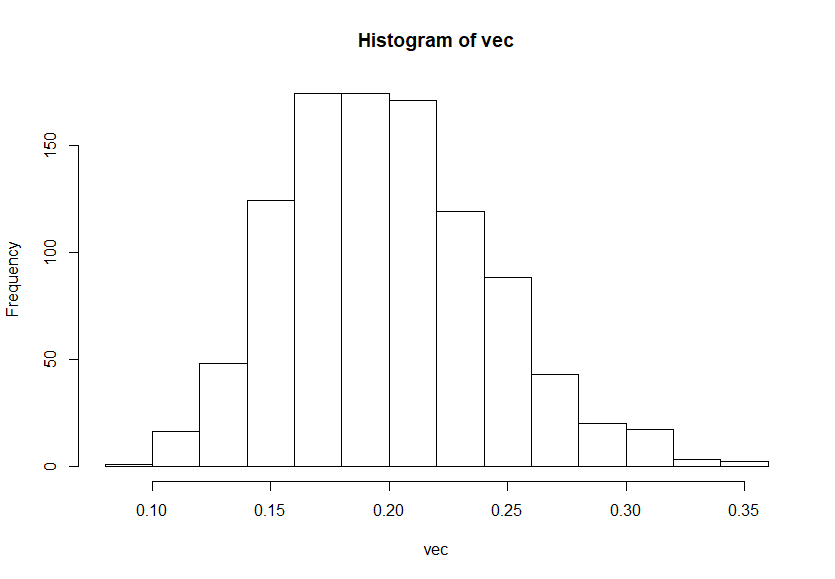
\includegraphics[scale =.5]{Rplot.png}
	\end{figure}
	\end{enumerate}
\end{enumerate}

\end{document}
